\documentclass{beamer}
\hypersetup{colorlinks=true,linkcolor=red}
\usetheme{Luebeck}
\useoutertheme[subsection=false]{smoothbars}
\useoutertheme{umbcfootline}

\usepackage{listings}
\definecolor{eclipse-red}{RGB}{127,0,65}
\definecolor{eclipse-green}{RGB}{63,127,95}
\definecolor{eclipse-blue}{RGB}{42,0,255}
\definecolor{eclipse-gray}{RGB}{100,100,100}
\lstset{language=Java,
        basicstyle=\scriptsize\ttfamily,
        keywordstyle=\color{eclipse-red},
        commentstyle=\color{eclipse-green},
        stringstyle=\color{eclipse-blue}\slshape,
        showstringspaces=false,
        escapechar=\$,
}


%--- Metadata -------------------------------------%
% Audience:      master students at computer science and engineering department
% Time budget:   30 min talk + 15 min questions + 15 min break
% Sructure:      start from general, go into details, leave 2-3 min for conclusions
% Thesis title:  Code coverage criteria and their effect on test suite qualities
% Goal:          Present our work, i.e. what we have done
\title{Code coverage criteria and their effect on test suite qualities}
\author[M.Kalkov \and D.Pamakha]
{\texorpdfstring
  {\begin{columns}
     \column{.45\linewidth}
     \centering
     Mikhail Kalkov\\
     \href{mailto:mikhail.kalkov@gmail.com}{\texttt{\small mikhail.kalkov@gmail.com}}
     \column{.45\linewidth}
     \centering
     Dzmitry Pamakha\\
     \href{mailto:pomaxodv@gmail.com}{\texttt{\small pomaxodv@gmail.com}}
   \end{columns}}
  {Mikhail Kalkov \and Dzmitry Pamakha}
}
\institute[Chalmers University of Technology]{
  Master Programme in Software Engineering and Technology\\
  Computer Science and Engineering Department\\
  Chalmers University of Technology\\
  Gothenburg, Sweden
}
\date[December 2013]{December 17, 2013}

\begin{document}

%--- Title frame ----------------------------------%
\begin{frame}[plain]
  \titlepage
\end{frame}

%--- Contents -------------------------------------%
\frame{
  \frametitle{Contents}

\tableofcontents
}


%--------------------------------------------------%
\section{Introduction}

%--------------------------------------------------%
\subsection{Motivational example}

%--- Frame ----------------------------------------%
\begin{frame}
  \frametitle{Motivational example}
\begin{columns}[T]
\begin{column}<2->{.5\textwidth}
  \centering
    Some program\\
    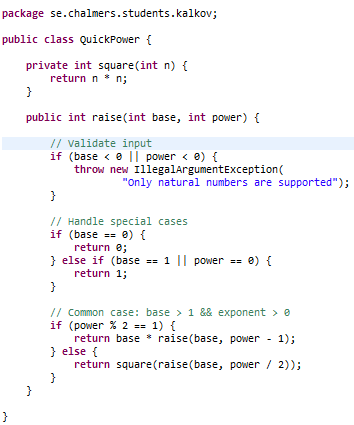
\includegraphics[scale=0.5]{QuickPower.png}
\end{column}
\begin{column}<3->{.5\textwidth}
  \centering
    Unit tests\\
    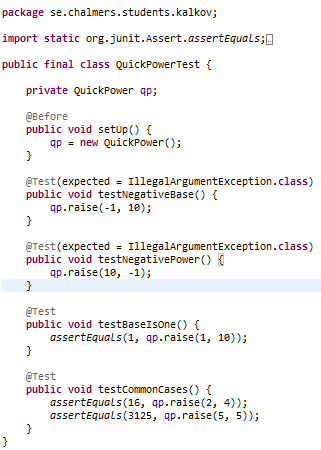
\includegraphics[scale=0.5]{QuickPowerTest.png}
\end{column}
\end{columns}
\end{frame}

%--- Frame ----------------------------------------%
\begin{frame}
  \frametitle{Motivational example}
\centering
How do you know that you have not forgotten to test some behaviour?
\end{frame}

%--- Frame ----------------------------------------%
\begin{frame}
  \frametitle{Motivational example}
\centering
It turns out many people use \emph{code coverage analysis} to answer this question.
\pause
\begin{columns}[T]
\begin{column}{.5\textwidth}
  \centering
    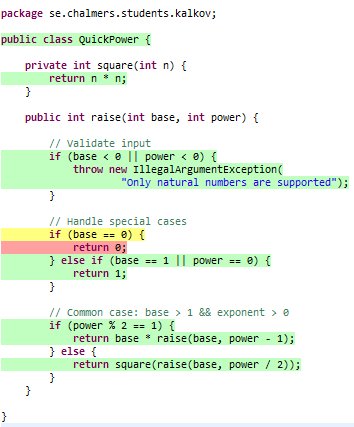
\includegraphics[scale=0.5]{QuickPower_colored.png}
\end{column}
\begin{column}{.5\textwidth}
  \centering
    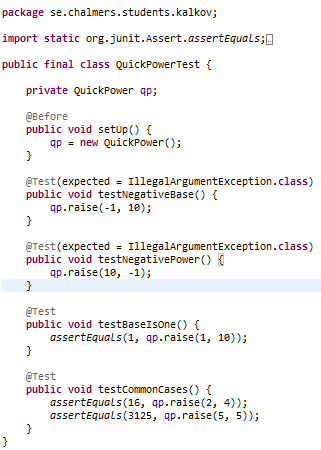
\includegraphics[scale=0.5]{QuickPowerTest.png}
\end{column}
\end{columns}
\end{frame}

%--------------------------------------------------%
\subsection{Research questions}

%--- Frame ----------------------------------------%
\begin{frame}
  \frametitle{Research questions}
\begin{itemize}
  \item What are common coverage criteria and their limits of applicability?
  \pause
  \item Which test suite qualities can be measured or affected by utilizing code coverage data?
  \pause
  \item What are common ways to present code coverage data and do they faithfully reveal
important test suite qualities?
  \pause
  \item How to implement an Eclipse plug-in for BullseyeCoverage so that code coverage data
can be fully utilized?
\end{itemize}
\end{frame}


%--------------------------------------------------%
\section{Coverage criteria}


%--------------------------------------------------%
\section{Test suite qualities}


%--------------------------------------------------%
\section{Coverage visualization}


%--------------------------------------------------%
\section{Bullseye plug-in for Eclipse}


%--------------------------------------------------%
\section{Conclusion}


%--------------------------------------------------%
\section{Discussion}

%--- Frame ----------------------------------------%
\begin{frame}
\begin{center}
  Thank you for attention!\\
  It is discussion time now.
\end{center}
\end{frame}

\end{document}

